%\documentclass[fontsize=11pt, appendixprefix=true]{scrreprt}
\documentclass[11pt]{report}
\usepackage{tocloft}
%\renewcommand{\cftpartleader}{\cftdotfill{\cftdotsep}} % for parts
%\renewcommand{\cftchapleader}{\cftdotfill{\cftdotsep}} % for content
\renewcommand{\cftsecleader}{\cftdotfill{\cftdotsep}} % for sections, if you really want! (It is default in report and book class (So you may not need it).

% appendixprefix: hogy odaírja, hogy "Függelék A", ne csak "A"
%\usepackage[english, magyar]{babel}                        % nyelvi csomag
\usepackage[T1]{fontenc}                                   % ékezetes betűknél is legyen automatikus elválasztás
\usepackage[utf8]{inputenc}                                % ékezetes betűk kezelése
%\usepackage{lmodern}                                       % alapértelmezett betűtípus ne legyen pixeles
%\usepackage{mathtools}                                     % képletekhez kell
\usepackage[backend=biber, sorting=anyt]{biblatex}           % bibliográfia
\usepackage{parskip}
\addbibresource{projectlab.bib}
\usepackage{url}
\usepackage{enumitem}
\usepackage{amsmath}
\usepackage{amssymb}
\usepackage{graphicx}                                      % képek beszúrása
%\usepackage{subcaption}
\usepackage{subfig}
\graphicspath{ {images/} }
\usepackage[export]{adjustbox}                             % ez az ITK logó pozicionálásához kell
\usepackage[margin=2.5cm, bindingoffset=1.25cm]{geometry}  % margók
\usepackage[onehalfspacing]{setspace}                      % másfeles sorköz
\usepackage[hidelinks, unicode, pdfusetitle]{hyperref}     % kattintható tartalomjegyzék és hivatkozások
\usepackage{bookmark}                                      % PDF könyvjelzők
\usepackage{csquotes}                                      % a bibliográfiában megfelelően legyenek formázva az idézőjelek
\DeclareQuoteAlias{german}{magyar}
\usepackage{blindtext} %mer mért ne?
% Kódrészletekhez ajánlom
\usepackage{listings, scrhack}
%\usepackage{sourcecodepro} % egy jó betűtípus
\lstset{captionpos=b, numberbychapter=false, basicstyle=\ttfamily, showstringspaces=false, columns=fullflexible}
% Kódrészletek magyar stílusú számozása
%\renewcommand\lstlistingname{kódrészlet}
%\makeatletter
%\renewcommand\fnum@lstlisting{\ifx\lst@@caption\@empty\else\thelstlisting.~\fi\lstlistingname}%
%\makeatother
% Nyilatkozathoz két parancs definíciója
\newcommand{\pushtobottom}{\vspace*{\fill}}
\newcommand{\signatureline}[1]{\begin{flushright}
	\vspace*{.5cm}\par\noindent\makebox[2.5in]{\hrulefill}
	\par\noindent\makebox[2.5in][c]{#1}
	\end{flushright}
}

% reference
\usepackage[plain]{fancyref}
%\usepackage[english, nameinlink]{cleveref}

%formázás

\usepackage{fancyhdr}
\pagestyle{fancy}
\fancyhf{}
%\fancyhead[L]{\leftmark}
\fancyhead[L]{\textsl{\rightmark}}
\fancyhead[R]{\thepage}
\renewcommand{\headrulewidth}{.001cm}

% Ezeket írd át!
\author{Csaba Botos}
\title{
AF Classification from a short single lead ECG recording:\\
the PhysioNet/Computing in Cardiology Challenge 2017
}
\date{2016}

\usepackage{titlesec}

% Chapter customization
\renewcommand\thesection{\arabic{section}}
\setcounter{secnumdepth}{2}

\titleformat{\chapter}[block]
  {\normalfont\Huge\bfseries}{\thechapter.}{1em}{\huge}
%\titleformat{\subsection}[block]

% For quotes
\usepackage{epigraph}
\setlength\epigraphwidth{0.7\textwidth}
\setlength\epigraphrule{0pt}

\begin{document}
%%%%%%%%%%%%%%%%%%%%%%%%%%%%%%%
%% BEVEZETÉS


\includegraphics[valign=m]{ITK_logo} \parbox[c]{0.8\textwidth}{
Pázmány Péter Catholic University\\
Faculty of Information Technology and Bionics}
\vspace*{\fill}

{\let\newpage\relax\maketitle}
\vspace*{\fill}
\begin{center}
A review submitted in partial satisfaction of the requirements of Individual
laboratory
\bigskip

Advisor: PhD.\ István Z. Reguly \\
\end{center}
\clearpage


\pagenumbering{Roman}
\section{Abstract}
Atrial Fibrillation is the most common type of cardiac arythmia.

ötletek még abstracthoz

http://www.sciencedirect.com/science/article/pii/S1746809413000062

https://physionet.org/challenge/2017/

\addcontentsline{toc}{chapter}{Abstract}

\pagenumbering{arabic}
\chapter{Introduction}
\section{Overview}


\epigraph{\textit{No one knows what the right algorithm is, but it gives us hope that if we can discover some crude approximation of whatever this algorithm is and implement it on a computer, that can help us make a lot of progress.}}{\rightline{{\rm --- Andrew Ng}}}

Every time we are interacting with our environment, we get closer to understanding it. %still the closer we are the less we understand. 
However, as a byproduct, further questions arise, for which pure logical (or mathematical) solution is not available, or the problem is larger than what we can solve.
Luckily we can always turn back to nature for inspiration: biological systems have proven their efficiency, therefore their functions are worth to be further analyzed -- even if there could be theoretically a better way to tackle obstacles. 
One of the many branches of artificial intelligence, Neural Networks are based on the nervous systems of living organisms which is capable of self-learning.

Such a simple paradigm is playing a fundamental role in boosting 
industry and research of today, because introducing Machine Learning to many fields of life seems to results in great leap forward. 
Thanks to the recent technological advancements, even with the current computational capacity of a personal computer one can get encouraging results by simply exploring the core principles of the topic. 

In this work I provide a detailed explanation of each step of building a library,
which is capable of reproducing current results of scientific researches.
Also present applications which were made with my own library and case studies in which I have achieved unique results.
Finally I propose the main innovation of my recent work: a simple algorithm for visualizing the \textbf{perceptive field} of each layer in a feed-forward network.

\paragraph{Primary goal.} With my work I intend to bring closer, and demystify cutting-edge concepts of applied neural networkings for larger audiences. 
On related works and case studies I want to show what can be done by simply going back to the drawing board

\clearpage
\section{Related Works and Literature}

\paragraph{Main motivation.} By using external libraries \cite{TF, torch, caffe}, without diving deep into mathematical proofs, and treating neural networks as black-boxes, thousands of useful applications \cite{haykin2004comprehensive} are made. 
On the other hand, building such architectures from the very basics helps to clarify how simple units might be organized~\cite{milo2002network}, taught \cite{werbos1994roots}, and function \cite{hornik1989multilayer} as a large system. 
As complexity arises, the processes in the network becomes unclear and brings the question: what is the purpose of each node? 
Methods to visualize how activation patterns formulate, and what information is held within them has been already investigated \cite{yosinski2015understanding}, and applied to improve performance \cite{zeiler2014visualizing}. 
My studies mainly rely on recent publications, and research in field of computer vision. The design of my own Deep Learning framework library is influenced by off-the-press tutorials \cite{Goodfellow-et-al-2016-Book, deeplearningdotnet, nnsdl, stanfordlectures, gibiansky} and open-source libraries \cite{TF, torch, caffe} available to anyone.

Considering course slides \cite{stanfordlectures, oxfordlectures} and textbooks \cite{Goodfellow-et-al-2016-Book, werbos1994roots, bengio2009learning} of established universities, popular websites \cite{deeplearningdotnet, pedregosa2011scikit}, 
articles \cite{lecun2015deep}, blogs \cite{gibiansky, karpathyblog} and vlogs \cite{vlog1} on Artificial Neural Networks one might find it hard to find a good point to start. 
Some content may offer formal description of the general machine learning problem, others try to clarify through analogies with the biological nerve system.
Tutorials, which I have found interesting, and the most helpful, had several common features which are important to adapt, when designing a neural network library.
Generally these common attributes are the following: 
they intend to be \emph{simple} as possible, 
have many \emph{intuitive} examples and analogies,
their \emph{interpretations} are not restricted to either universal approximators, 
or nervous systems of living organisms, but combines both aspect.

I have written the first implementation based on chapters of \cite{nnsdl}. 
What I have understood is the basic forward- and back-propagation \cite{werbos1994roots} concept of neural networks.
Since I was struggling to understand the coding tricks that the author involved 
I could not extend the source to any problem.
I decided to work out the mathematical formulation, to re-implement feed-forward networks from the beginning.
Reading a practical guide~\cite{karpathyblog} pointed out how can we represent \emph{gradient flow}, \emph{computational graphs} in a simple way.
His style of explaining complex theoretical concepts through very clear examples motivated me to
write my own guide which covers those parts that I was missing from the literature mentioned above.

When the library was working, the next step was writing demo applications, in which I have experimented with hyper-parameters.
These applications were based on \emph{Browser demos} of \cite{convnetjs}.
In this work only two of them is present, which are related to visualization.
Later I was experimenting with different methods of revealing the \emph{perceptive field}.
In \cite{breakingclass} I learned about how modern networks can be fooled with \emph{adversarial samples} which referred to \cite{goodfellow2014explaining} and \cite{nguyen2015deep}. 
Further investigation in the area revealed basic methods on understanding how each neuron works in a network \cite{yosinski2015understanding}.
I was inspired to develop my own algorithm while I was studying the novel architecture of DeconvNets \cite{zeiler2014visualizing}.

\clearpage
\section{Thesis outline and contributions}
In this work I summarize my recent studies on Neural Networks and Computer 
Vision. 
I present my current achievements in the field, the visualization 
techniques I have derived and developed from the latest 
self-educational sources and novel research.
I also provide a guide on how to build a library \textbf{from scratch} 
which I used for producing the present results.


In Chapter \textbf{\nameref{cp:design}} I explain the overall structure of the library and the considerations which led to them, and provide a detailed explanation on how I 
derived the main concepts of neural networks, from the very beginning supported with mathematical background. 
First I zoom in from a larger picture of working AI to exact challenges of 
Machine Learning: I disassemble neural networks in general, to basic 
building blocks, explain them through several examples and provide a 
formal mathematical definition which will be used in the following 
sections.
I put emphasis on linking the formal definitions to natural meanings of 
mathematical formulas (throughout rather informal explanations).
By providing intuitive theoretical considerations, from the perceptron 
model, I build up step-by-step the entire idea of \emph{Forward- \& 
Back-propagation} of Deep Neural Networks.
In the end, exact layers are described involving examples of practical applications.

In \textbf{\nameref{cp:results}}, I describe my research on 
visualization techniques via elementary case studies of \emph{Voice 
Recognition} and \emph{Image Classification}.
In the first half I summarize the main concepts and capabilities of single 
layered neural networks.
I start with the basic problems of voice recognition, namely the 
overlapping frequency domains, the irrelevant signals (noise) by training 
networks on pure sinusoid input samples.
I provide examples for the problem of overfitting and show how regularization techniques enhances the network performance.
After clarification, I explain the challenges of the voice recognition topic involving real recordings,
a case study that can be carried out at home by anyone, with the knowledge 
provided by my work.
In the second half, I show how feed-forward networks can be better understood via visualization with a simple algorithm, namely the \emph{Gradient Ascent}, which I have developed based on my previous studies of novel articles.
I have also explored the hyper-parameter space of fully connected architectures,
while training networks on the popular MNIST dataset.
I present my experiments with different shape of layers and methods for training, and share my interpretations of the results.
In the end an exhaustive investigation of different types of Gradient Ascent can be found involving research of revealing perceptive field of neuron each neuron in a given layer and generating adversarial samples from any kind of input which can be used for harnessing the network.

Finally, in the last chapters I summarize the research I have done so far and discuss the path forward.





%
%\section*{Biological Motivation}
%\section*{Real Life Applications}
%\section*{Black Box representation}
%\section{The Perceptron model}
%\section{Importance of understanding}
%\section{Visualization}

%% BEVEZETÉS
%%%%%%%%%%%%%%%%%%%%%%%%%%%%%%%
%% TARTALOM
\chapter{Related Works}

ez még maradhat a végére

\section{Differentiation}\label{sec:diff}
In the above evaluating of $\nabla_\phi \mathcal{F}$ can be done in two ways, namely by numerical approximation, or by analytical derivation, in the following I will discuss both.

\subsection{Numeric differentiation} Evaluating the numerical gradient (or difference) is an elementary, yet powerful operation, in which we would \emph{perturb}, or modify one parameter $\phi$ of our system $\mathcal{F}$ at once.
That is done by first adding $\phi^+$ and after subtracting $\phi^-$ a little amount $d\phi$ from the original $\phi$ and evaluate $\mathcal{L}^{\pm}=\mathcal{L}(\mathcal{F}_{\phi^{\pm}})$, namely the \emph{Loss} of the system in the modified state, yielding the numerical gradient in the following equation:

\begin{equation} \label{eq:numgrad}
    \frac{d\mathcal{L}(\mathcal{F})}{d\phi} = 
    \frac{\mathcal{L}^+ - \mathcal{L}^-}{2 d\phi} = 
    \frac{\mathcal{L}(\mathcal{F}_{\phi^+}) - \mathcal{L}(\mathcal{F}_{\phi^-})}{2 d\phi}
\end{equation}

\paragraph{Summary.} In a nutshell value of $\frac{d\mathcal{L}(\mathcal{F})}{d\phi}$ tells how changing the parameter $\phi$ by $d\phi$ would change the performance of the network. If it is positive then updating $\mathcal{F}$ by adding $d\phi$ to $\phi$ would result in higher Loss value, which is the opposite of our goal, so we just subtract it, if it is negative, then trivially we should add $d\phi$ to $\phi$ since it is making some good progress.

\subsection{Complexity} 
Though letting the computer do the hard work seems to be a good idea, it is worth considering that the simple method above will be applied to every $\phi$ of $\mathcal{L}$.
It means that for the network in the toy example, we need to evaluate $\mathcal{L}(\mathcal{F})$ two times for each parameter in 
the weight matrices and the bias vectors of the network, totaling in 
$$\#(\phi) = 2\times\sum_{i=1}^3 N_{(i-1)}\cdot N_i + N_i = 2\times(10\cdot 5 + 5 ... + 4\cdot 3 + 3) = 188$$
Even if $\mathcal{F}$ is approximated by using $k$-sized mini-batches for evaluation it is still a computationally very expensive function, because the inference would result in the following number of operations of addition and multiplication:
$$\#(\mathrm{operations}) = k\times\sum_{i=1}^3 2\cdot N_{(i-1)}\cdot N_i + N_i = k \times 176$$
Therefore approximated with $k=10$ mini-batches would a single parameter update of a very tiny network would require total operations of:
\begin{equation}
    \#(\mathrm{total})=\#(\phi) \times k \times \#(\mathrm{operations}) = 188 \cdot 10 \cdot 176  = 330880
\end{equation}
Because both $\#(\phi)$ and $\#(\mathrm{operations})$ has complexity of $\mathcal{O}(N^2)$, one update will yield complexity of 
\begin{equation}
    \#(\mathrm{total})=\mathcal{O}(N^4)
\end{equation}
We can see that even for a shallow and relatively small network (industrial AI networks has billions of parameters, and uses much larger batches) described in the toy example the method is really costly.
That encourages us to derive our differentials on paper first, and use \emph{numerical gradient approximation} for checking our solution. Using \emph{Gradient Check} is essential when implementing new architectures, because it is a very efficient tool for debugging in comparison with updating. The method in a few words is about setting an error rate $\epsilon$, and decrease $d\phi$ until the numeric solution does not match the analytic solution with $1-\epsilon$ significance. If the analytic solution is incorrect the cycle will not terminate.

\subsection{Analytic differentiation}
Deriving the update by hand requires basic knowledge in calculus extended to multivariate cases, though since the operations are elementary, in general we must understand only three basic definitions to do so. 
Some formality before starting: we have three independent variables $x$, $y$, $z$ and functions $f$, $g$, $h$. The result of operations performed on variables, i.e. $x+2y$ can be represented by a function $f=x+2y$. 
If the value depends on a variable then it can be written explicitly, passing the variable as \emph{the argument} of the function $f(x,y)=x+2y$. 
For the sake of simplicity assume that the variables are not general objects from an abstract space, they are only real values: $x,y,z\in \mathbb{R}$. However the following description could be extended for the above-mentioned variables as well. For any one-dimensional function $f(x):\mathbb{R}\mapsto\mathbb{R}$ we say that the value represented by the function depends on the variable by the extent of its derivative. The derivative (or differential) of the function can be seen as an ideal case of \ref{eq:numgrad} where the perturbation would approach zero, namely:
\begin{equation}
    \frac{\partial f}{\partial x} = \lim_{dx\rightarrow 0}\frac{df(x)}{dx}= \lim_{dx\rightarrow 0} \frac{f(x+dx)-f(x-dx)}{2dx}
\end{equation}
\paragraph{Multiplication rule.}
Consider a value $x\cdot y \cdot z$ represented by $f(x,y,z)$. $f$ is now depending on three variables, we can define the measure of this dependency on one variable by the formal equation:
\begin{equation*}
\begin{split}
    \frac{\partial f}{\partial x} = \lim_{dx\rightarrow 0} \frac{f(x+dx,y,z)-f(x-dx,y,z)}{dx}
    &= \lim_{dx\rightarrow 0} \frac{((x+dx)\cdot y \cdot z)-((x-dx)\cdot y \cdot z)}{2dx} \\
    = \lim_{dx\rightarrow 0} \frac{(x+dx)-(x-dx)}{2dx} y z&= \lim_{dx\rightarrow 0} \frac{2dx}{2dx} yz= yz
\end{split}
\end{equation*}
We can apply the same method for each variable, the result will be the elements of the \emph{gradient} $\nabla f$
\begin{equation}\label{eq:multiplication}
    \frac{\partial f}{\partial x} = y z \qquad
    \frac{\partial f}{\partial y} = x z \qquad
    \frac{\partial f}{\partial z} = x y 
\end{equation} 
The important thing to understand that in a computational graph, a multiplicative node, which takes $N$ arbitrary parameters (or arguments), will have a \emph{partial derivative} for each variable its output is depending on. In general if these derivatives are represented as a vector, then it is called the gradient $\nabla f$ of $f$. Also the value of the derivative will be the product of all variables except the one of which we are computing the influence of on the output.

\paragraph{Addition rule.}
Consider a value $x\cdot y + x\cdot z$ represented by $g(x,y,z)$.
The change of $g$ with respect to $x$ is defined with the following shortened equation:
\begin{equation}\label{eq:addition}
    \frac{\partial g}{\partial x} = \lim_{dx\rightarrow 0} \frac{((x+dx)y +(x+dx)z)-((x-dx)y +(x-dx)z)}{dx}=y+z
\end{equation}
Notice that -- in the terms of computational graphs -- if a node contributes to other different operations (namely $x\cdot y$ and $x\cdot z$), 
than the derivative of each occurrence in \emph{later} values will be summed up. 

\paragraph{Chain rule.}
Let $f(x)=2x+3$ and $g(f)=5f$. Suppose that we would like to know the derivative of $g$ with respect to $x$.
At first we cannot do so, but there are two options: in the hope that substituting the value represented by $f$ into $g$ would not make the equation too complex we can unroll the references and rewrite $g(x)=5\cdot(2x + 3)$, or we could use the chain rule:
$$
    \frac{\partial g}{\partial x} = \lim_{dx \rightarrow 0} \frac{g(f(x+dx)) - g(f(x-dx))}{2dx}
$$

\begin{center}
    Assume that $f(x+dx)-f(x-dx) \neq 0$.
\end{center}

$$
    \lim_{dx \rightarrow 0} \frac{g(f(x+dx)) - g(f(x-dx) ) }{f(x+dx)-f(x-dx)} \cdot \frac{f(x+dx)-f(x-dx)}{2dx}
$$

\begin{equation}\label{eq:chain}
    \frac{\partial g}{\partial x} = \frac{\partial g}{\partial f} \cdot \frac{\partial f}{\partial x}
\end{equation}

Which is a formula of the products of partial derivative of $g$, that treats $f$ like a variable, and $f$ explicitly operating on variable $x$.
The derivative of $g$ with respect to variable $x$ is the product of the \emph{local derivative} of $g$ is $\frac{\partial g}{\partial f}=5$ and $\frac{\partial f}{\partial x}=2$ which equals $\frac{\partial g(x)}{\partial x}=\frac{\partial(5\cdot (2x + 3))}{\partial x} = 10$, the function strictly depending on $x$.
The important message is that we can interchangeably use function values and variables with a constraint that at a point, in an arbitrary depth there must be a real variable.
\emph{Note:} the statement above stands for computations with \emph{Acyclic Graph}, meaning that there should not be any feedbacks or loops -- no definitions like $f(g), g(f)$ or $f(f)$.
We will see that these rules play a very fundamental role in training networks.

\paragraph{Vector Notation.}
Before drilling deep into mathematical equations, a small reminder: the following vector and matrix formulation is just a special annotation, 
using the rules above, which helps to make clear both the definition, and the computations done by the network when it is implemented. 
The vectors with partially derivatives inside are just representing \emph{real values}, arranged in a fancy way.
Every vector and matrix defined in forward propagation, has its corresponding derivative w.r.t. the Loss.
More trivially, if any value is depending on a list of variables $f(x_1, x_2 \cdots x_n) = f(\mathbf{x})$ (a vector) then there is a list of \emph{partial derivatives} w.r.t. to $f$ -- forming the gradient $\nabla f = \left(\frac{\partial f}{x_1}, \frac{\partial f}{x_1} \cdots \frac{\partial f}{x_N}\right)$. 
\emph{Notation}: When the vector notation is emphasized the variable name is conventionally written in bold font $\mathbf{x}$, or is underlined \underline{$x$}.
Because later the indexing would become too crowded, we only use the indexed notation when it is necessary, otherwise using $x$.

The next step is formulating the dependency of multiple functions on multiple variables.
As seen above, a multivariate function has its gradient vector --
in the same fashion as the list of variables were organized into vectors $\mathbf{x}$, values composed of them can also form a vector $F = (f_1, f_2 \cdots f_M)$, composing a multivalued function depending on the same variables.
Doing so yields a first-order derivative matrix, composed of gradient vectors $J=(\nabla f_1, \nabla f_2 \cdots \nabla f_M)^T$, called the \emph{Jacobian of $F$}.
The Jacobian has as many rows as output values $F$ has, and the same number of columns of the variables that $f_i$ is a function of.
\begin{equation}\label{eq:jacobian}
    J(F) = 
    \begin{pmatrix}
    \quad \nabla f_1 \quad \\ 
    \vdots \\ 
    \nabla f_M
    \end{pmatrix} 
    =
    \begin{pmatrix}
    \frac{\partial f_1}{\partial x_1} & \cdots & \frac{\partial f_1}{\partial x_N} \\ 
    \vdots & \ddots & \vdots \\ 
    \frac{\partial f_M}{\partial x_1} & \cdots & \frac{\partial f_M}{\partial x_N}
    \end{pmatrix} 
\end{equation}
The matrix and vector operations (such as addition and inner product) that can be performed on the derivative \emph{arrays} are identical defined in the inference section. That is important because product of derivatives introduced by the chain rule, can be applied as well for multidimensional array of derivatives too.

\subsection{Fully Connected Layer}
Return to the toy example and begin with the last layer, with $3$ nodes. If a sample $x$ is inferred $\mathcal{F}(x)=y$, then the response of the network will be a vector of $dim(y) = 3$. If we took the $L_2$ \emph{distance} between the response and the goal $y^*$, then it would tell how far we are from the ideal, by a single scalar value. Since we want to minimize it, we have to adjust the parameters of the network, namely descend on the gradient slope. To get the small extent of the update we have to evaluate $\frac{\partial\mathcal{L}}{\partial \phi}$. 
Intuitively in the case we would like to correct the weights of a decision, it would require two things:
\begin{itemize}
    \item[] The original situation (the input of the $l^{th}$ layer $x_l$), which the decision was made in.
    \item[] The error on the decision -- the derivative $\delta^l$ of the Loss with regards to the decision.
\end{itemize}
Since $x_l$ is obtained via inference, what we have to calculate is $\delta^l$ for the $l^{th}$ layer in order to acquire the parameter gradient.
The first step is to evaluate the $\delta_L$, or the \emph{error} of the last layer's response $y^3$, namely $\delta^3 = \nabla_{y^3} \mathcal{L}$.
Begin with the first element: 
$$
    \delta_1^3 = 
    \frac{\partial \mathcal{L}}{\partial y_1} = 
    \frac{\partial}{\partial y_1}\frac{1}{2}\left((y^*_1 - y_1)^2 + (y^*_2 - y_2)^2 + (y^*_3 - y_3)^2\right) = y_1 - y^*_1
$$
\begin{center}
Expanding it to the whole array:
\end{center}
$$
    \delta^3 = \begin{pmatrix}
     \frac{\partial \mathcal{L}}{\partial y_1}\\ \\
    \frac{\partial \mathcal{L}}{\partial y_2} \\ \\
    \frac{\partial \mathcal{L}}{\partial y_3}
    \end{pmatrix} = \begin{pmatrix}
     \frac{\partial}{\partial y_1} \frac{1}{2}\sum_i(y_i^*-y_i)^2\\ \\
    \frac{\partial}{\partial y_2} \frac{1}{2}\sum_i(y_i^*-y_i)^2 \\ \\
    \frac{\partial}{\partial y^3_3}  \frac{1}{2}\sum_i(y_i^*-y_i)^2
    \end{pmatrix} = \begin{pmatrix}
     {y_1-y^*_1}\\ \\
     {y_2-y^*_2}\\ \\
     {y_3-y^*_3}
    \end{pmatrix} 
$$
Consider the following notation:
$
    \delta^3_i = (y^*_i - y_i)
$, 
called parametric vector notation. Writing arrays in this way, saves a lot of space. However, when this notation gets jammed with indexes, it is useful to write down explicitly the whole array for clarification.

\paragraph{The last layer} Now we have exact values of $\delta^3$ and $x^3$, so we can calculate how should the weights in $W^3$ be changed in order to get a better network.
Applying the differentiation rules for each weight (forming a matrix) of the layer will result in a derivative for each weight (also forming a matrix).
Taking the first perceptron of the layer, it has a weight $W^3_1=(W_{1,1}, W_{1,2}, W_{1,3}, W_{1,4})$ for each output of the previous layer.

Suppose that this neuron had to tell how rounded is the object on an image sample, 
and the $i^{th}$ neuron of the $2^{nd}$ layer fires when it recognizes sharp edges.
Of course it would be bad if our neuron had a large weight on $x^3_i$. 
If this node performs poorly because of $x^3_i$, then it would contribute a lot to the Loss function while inferring sharp objects, with its output $y_1$ being far away from $y^*_1$, resulting in a positive $\delta^3_1$. 
In case of $x^3_i = 0$, the weight $W_{1,i}$ has nothing to do with the error $\delta^3_1$ of the neuron.
Notice that the error of each weight (w.r.t $\mathcal{L}$) should be proportional to the error and the input as well: $\frac{\partial \mathcal{L}}{\partial w_{1,i}}=x^3_i \cdot \delta^3_1$.
However it can be also derived in terms of the differentiation rules: 
$$
    \frac{\partial \mathcal{L}}{\partial W_{1,i}}=
    \frac{\partial \mathcal{L}}{\partial y^3_1}\cdot \frac{\partial y^3_1}{\partial W_{1,i}} =
     \delta^3_1  \cdot x^3_i
$$

\paragraph{Considering the parameter update.} assume that a picture of an origami sculpture (a very edgy one) was inferred and the $i^{th}$ node of the second layer worked correctly. Both $x^3_i$ and $\delta^3_1$ is positive, however the weight should be decreased: that is why we will take the negative of the derivative for updating $w_{1,i}$.
Substituting $i=1,2,3,4$ into $\frac{\partial \mathcal{L}}{\partial w_{1,i}}$ yields a gradient of $\mathcal{L}$ with regards to the weights of the first neuron of the last layer. 
Doing so for each neurons in the layer would result in 3 gradient vectors $\nabla_{W_1} \mathcal{L}$, $\nabla_{W_2} \mathcal{L}$ and $\nabla_{W_3 }\mathcal{L}$ which is practically stacked to make a matrix which can be later added element-wisely to the weight matrix $W$.
$$
\nabla_W \mathcal{L} = 
\begin{pmatrix}
\frac{\partial \mathcal{L}}{\partial W_{1,1}} & \frac{\partial \mathcal{L}}{\partial W_{1,2}} & \frac{\partial \mathcal{L}}{\partial W_{1,3}} & \frac{\partial \mathcal{L}}{\partial W_{1,4}} \\ \\
\frac{\partial \mathcal{L}}{\partial W_{2,1}} & \frac{\partial \mathcal{L}}{\partial W_{2,2}} & \frac{\partial \mathcal{L}}{\partial W_{2,3}} & \frac{\partial \mathcal{L}}{\partial W_{2,4}} \\ \\
\frac{\partial \mathcal{L}}{\partial W_{3,1}} & \frac{\partial \mathcal{L}}{\partial W_{3,2}} & \frac{\partial \mathcal{L}}{\partial W_{3,3}} & \frac{\partial \mathcal{L}}{\partial W_{3,4}}
\end{pmatrix} = 
\begin{pmatrix}
 x_1 \delta_1 &  x_2 \delta_1 &  x_3 \delta_1 &  x_4 \delta_1 \\ \\
 x_1 \delta_2 &  x_2 \delta_2 &  x_3 \delta_2 &  x_4 \delta_2 \\ \\
 x_1 \delta_3 &  x_2 \delta_3 &  x_3 \delta_3 &  x_4 \delta_3
\end{pmatrix}
$$

The last part of the equation can be also expressed as:
\begin{equation}
\nabla_W \mathcal{L} = \left(\frac{\partial \mathcal{L}}{\partial W_{i,j}}\right) = \left(x_j \delta_i\right) = x \wedge \delta
\end{equation}
Where $\wedge$ denotes the \emph{outer product} operator. 
The gradient of the bias is simply $\nabla_{b^L} \mathcal{L} = \delta^L$.

\paragraph{The $(L-1)^{th}$ layer.} Gradient descent can be applied on networks with more than one layer, 
however continuing the example of the image descriptor network requires a bit more abstraction. 
In the previous explanation we assumed that the $i^{th}$ neuron of the second layer worked properly.
In general cases this assumption is incorrect, if the whole network is initialized at once.
If we think about that also the mentioned neuron in the \emph{last hidden layer} should be trained, 
then we can apply the same method with a 4 dimensional $\delta^{(L-1)}$ and with a 5 dimensional $x^{(L-1)}$ input.

\emph{Note}: Capital $L$ is representing the number of layers. In the toy example $L = 3$.\\
Acquiring the $\delta^{(L-1)}$ is where the chain rule \eqref{eq:chain} steps into the scene.
While in the example before we could find an intuitive workaround, in this case it would be quite strained, since $\mathcal{L}$ does not depend directly on $y_{(L-1)}$.
Utilizing the chain rule:
\begin{equation}\label{eq:backward}
    \delta^{(L-1)} = 
    \frac{\partial \mathcal{L}}{\partial y^{(L-1)}} = 
    \frac{\partial \mathcal{L}}{\partial y^{L}} \cdot
    \frac{\partial y^{L}}{\partial y^{(L-1)}} = 
    \delta^L \cdot J(F_L)
\end{equation}
Where $J(F_L)$ denotes the \emph{Jacobian} \eqref{eq:jacobian} of the function representing the projection of the last layer $F_L:\mathbb{R}^4\mapsto \mathbb{R}^3$.
It is a map of how each input variable affects the output of the layer.
In general: the Jacobian numerically can be represented as a $3 \times 4$ matrix, analytically as a \emph{local derivative} of function $F$.
In case of \emph{Fully Connected} layers the Jacobian is simply the weight matrix $F(F_l)=W_l$ (the bias drops out here).

For derivative of scalar values ($\mathbb{R}$) the \emph{product} operator is well defined, 
and it can be expanded the same way to derivatives of multidimensional values as 
regular \emph{inner product} of the values they are composed of.
\emph{Note}: In order to stay consistent with the dimensions of the computation, we have to switch sides of the matrix multiplication defined in \eqref{eq:FC}:
\begin{equation}\label{eq:reverse}
\begin{split}
\delta^{(L-1)}_j &= 
    \sum_j \delta^L_i \; W^L_{i,j} \\
    \delta^{(L-1)} &= \delta^L \cdot W^L\\
    \left[4\right] &= \left[3\right] \cdot \left[3 \times 4\right] 
\end{split}
\end{equation}
\subsection{Backpropagation}
The backpropagation algorithm, first described by Werbos \emph{et. al} \cite{werbos1994roots}
\paragraph{The $l^{th}$ layer.} 
The contribution to the Loss of the general $l^{th}$ layer $\delta^l$ can be retrieved by unfolding $\frac{\partial \mathcal{L}}{\partial y^l}$ applying the chain rule, namely the backpropagation:
\begin{equation}\label{backprop}
\begin{split}
    \delta^l &= 
    \frac{\partial \mathcal{L}}{\partial y^{l}} = 
    \frac{\partial \mathcal{L}}{\partial y^{L}} \cdot
    \frac{\partial y^{L}}{\partial y^{(L-1)}} \quad \cdots \quad
    \frac{\partial y^{(l+1)}}{\partial y^{l}} \\
    \delta^l &= \delta^L \cdot J(F_L) \cdot J(F_{(L-1)}) \quad \cdots \quad J(F_{(l-1)})\\
    \left[dim(l)\right] &= \left[dim(L)\right] \cdot \left[dim(L)\times dim(L-1)\right] \cdots \left[dim(l+1)\times dim(l)\right]
\end{split}   
\end{equation}
\emph{Note}: the order of evaluating these derivatives is theoretically irrelevant, 
however computationally there is an opportunity to implement it in two ways \cite{akthesis}:
\begin{enumerate}
    \item[] \emph{forward-mode differentiation}: evaluating in the order of layers is efficient in cases where the output of the network is much larger than the input
    \item[] \emph{reverse-mode differentiation}: evaluating in reversed order for networks with fewer outputs than inputs.
\end{enumerate}
As pointed out in the thesis, the former would require $(L-l)$  times evaluating a \emph{matrix-matrix} product and one \emph{vector-matrix} operation,
while the latter would require $(L-l)$ times evaluating a \emph{vector-matrix} product and one \emph{matrix-matrix} at the end. 
Using forward-mode differentiation does not require keeping transient activations $y^l$, however it is computationally costly.
Using backward-mode differentiation does not strain the CPU, but the memory. 
It is because if $J(F_l)$ is not linear, then it requires the input $x_l$ to evaluate the first order derivatives.

\subsection{Activation Layer} 
Though the activation layer operates on the input, it has no adjustable parameter. 
Since we have to evaluate $\delta$ for layers behind activation layers, the error must pass through $J(F_{activation}$ as well.
Luckily activation layers applies a scalar function element-wise on the inputs, 
the Jacobian of the composite function $F$ has a special attribute: it is \textbf{diagonal}, meaning that:
$$
    J(F) = \frac{\partial F_i}{\partial x_j} = 
    \begin{cases}
        \frac{\partial f(x_i)}{\partial x_i} & i = j\\
        0 & i \neq j
    \end{cases}
$$
We can exploit this function when implementing activation layers, by simply using element-wise product $\frac{\partial f(x_i)}{\partial x_i}$ instead of a matrix multiplication.
The mentioned activation functions (\ref{eq:af1}, \ref{eq:af2}, \ref{eq:af3}, \ref{eq:af4}), are differentiable \emph{almost everywhere}, the corresponding derivatives:
\begin{align}
    \mathrm{(ReLU)' := } &\mathrm{Heaviside}(x)\\
    \mathrm{(TanH)' := }   & 1 - \tanh(x)^2\\
    \mathrm{(SP)' := }   &\frac{1}{1+e^{-x}}\\
    \mathrm{(Log)' := }  &\mathrm{Logistic}(x)\cdot (1-\mathrm{Logistic}(x))
\end{align}

\section{section name}

Evaluation of modells:

Separating the given set to -> train/eval/test

Because of unbalanced data -> extended precision recall -> Confusion Operator

Data augment -> trained on quasi-balanced totally augmented set

Data normalization -> BPM normalization through R wave detection with Pan Tompkins filtering -> invariant Time Features reveals

To make the network more sensitive on the rare samples of AF we introduced weighted loss training, where the mentioned samples yielded larger loss -> forcing the algorithm to categorize the undersampled classes more accurately.

\chapter{Benchmark of \texttt{filtfilt}}

In order to verify that my implementation of the \texttt{filtfilt} operator in TensorFlow is better for large scale applications than the publicly available state-of-the art method found in \texttt{SciPy.signal module}~\cite{scipy}, we attempted to measure the time required for evaluation.
For benchmarking purposes we used random sequences sampled from standard normal distribution.

I have prepared multiple test runs, where we compare the two methods by evaluation time concerning the sample length, the number of filters applied and the number of samples.

\section{Single sample - Single filter with different sample lengths}
In the first comparison the TensorFlow implementation performs poorly, we had to apply different $y$ label ticks.
The reason for this result, is that the implementation uses GPU acceleration via TensorFlow CUDA kernels, and the mobilization of the data (copying into the graphic memory, and copying the result out from it) takes more time than actually executing the operation.
Moreover, currently the TensorFlow backend does not support mutable \texttt{tf.Variables} inside native iterative loops \texttt{tf.while\_loop}, meaning that we cannot modify specific values by indexing an immutable \texttt{tf.Tensor}.
 In other words, \texttt{tf.Tensor} is the only interface for the inner body of the while loop that can communicate with external graph nodes.
Technically this yields, that the fixed size array of values cannot be allocated before the execution of an iteration, because the resulting space can only be handled by an interface that does not support element modification.
As a transient solution we had to include array concatenation, so in every step $t$ the array of previous outputs $[y_{1}, y_{t-1}]$ has to be concatenated to the current $y_t$ output value, resulting in memory expensive operations.

\begin{figure}[h]
  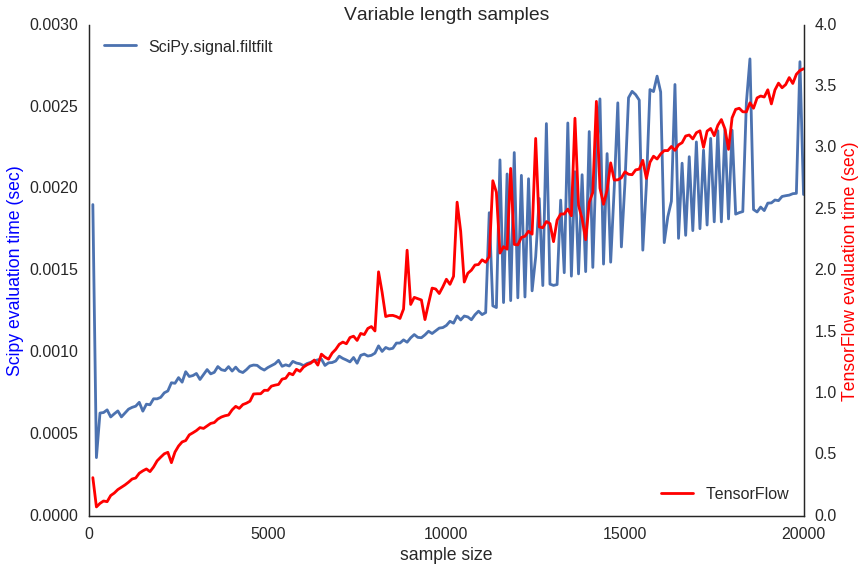
\includegraphics[width=.9\textwidth]{single}
  \caption{Time of evaluating a single sample with a single filter, at different sequence lengths. Later the measurement depicted with the blue line will be used as a baseline representing SciPy's performance on the given task. Notice that for we introduced a new axis for the TensorFlow implementation's time scale, because on single samples the performance of the two methods were not comparable.}
\end{figure}

\section{Batch of samples - Single filter run, with same length samples}

When multiple samples are available at run time, we can speed up the process, by running the same filter process in parallel.
Here we normalized the evaluation time per sample per filter of the SciPy method using the statistics of the previous experiment, since the method allows only processing in sequence, and after reproduced the standard SciPy baseline, to use as a reference point in further benchmarks, e.g. Figure~\ref{fig:batch}.
As we can see in Figure~\ref{fig:batch-tf-only}, the TensorFlow implementation runs in constant time at low batch size, and later starts to increase linearly

\begin{figure}
  \centering
  \begin{floatrow}
    \ffigbox[\FBwidth]{\caption{Comparison to the standardized SciPy baseline with regards to the baseline. The baseline is computed from the normalized average of the different sample length runs from the variable length single sample experiment. We show that with sample length 100, the current implementation only functions better when evaluation above 1500 sample at once.}\label{fig:batch}}{%
      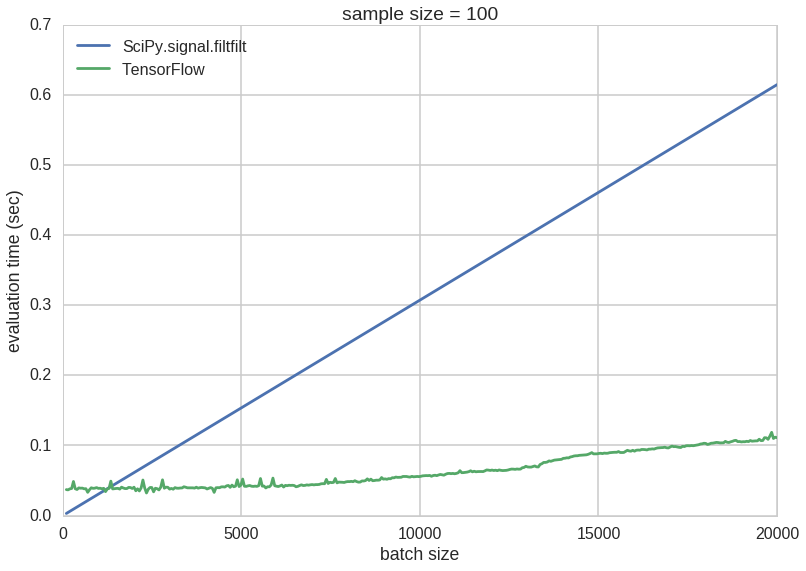
\includegraphics[width=.48\textwidth]{batch}
    }
    \ffigbox[\FBwidth]{\caption{Here only the TensorFlow implementation's evaluation time is depicted without the baseline. It reveals that under 4000 samples the process is nearly constant in time complexity. Above 2000 samples it starts to behave linearly, but it is important to mention that the slope of the fitting linear curve is significantly less steeper than the SciPy baseline.}\label{fig:batch-tf-only}}{%
      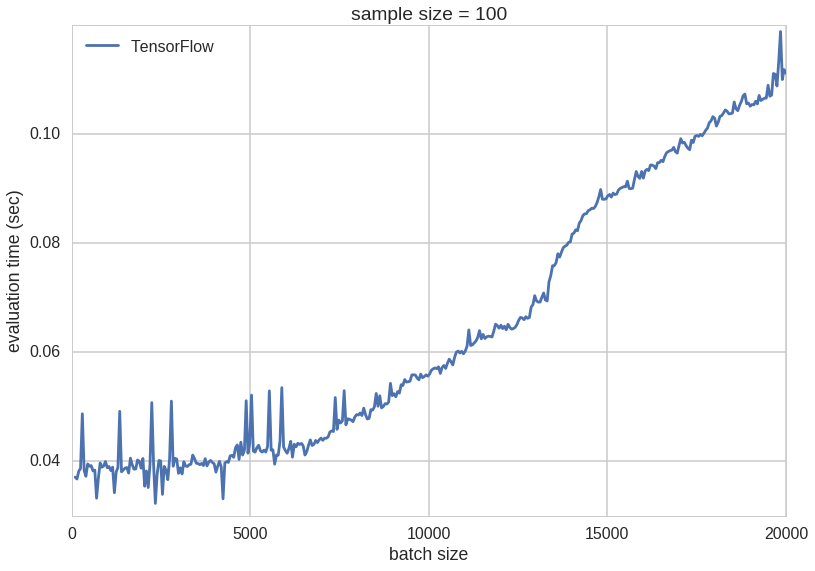
\includegraphics[width=.48\textwidth]{batch-tf-only}
    }
  \end{floatrow}
\end{figure}

% \begin{figure}
%   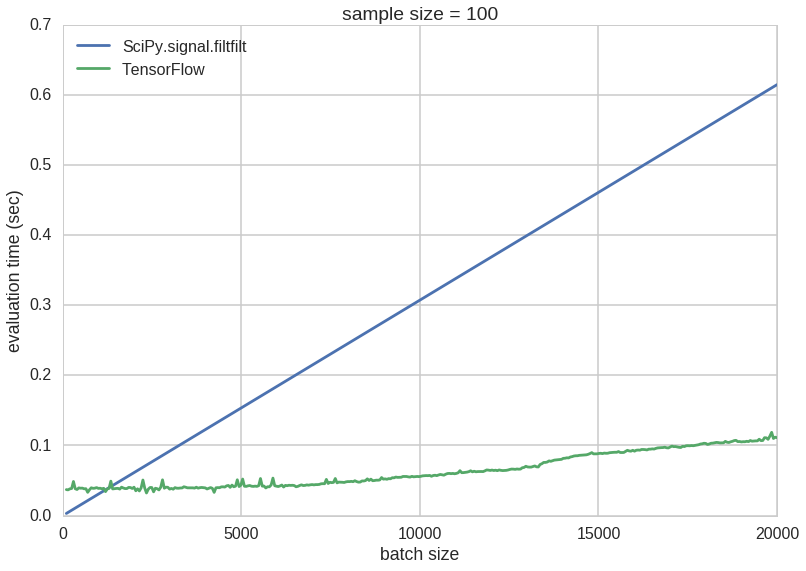
\includegraphics[width=.9\textwidth]{batch}
%   \caption{Comparison to the standardized SciPy baseline with regards to the baseline. The baseline is computed from the normalized average of the different sample length runs from Section~\ref{sec:single}}
%   \label{fig:batch}
% \end{figure}

% \begin{figure}
%   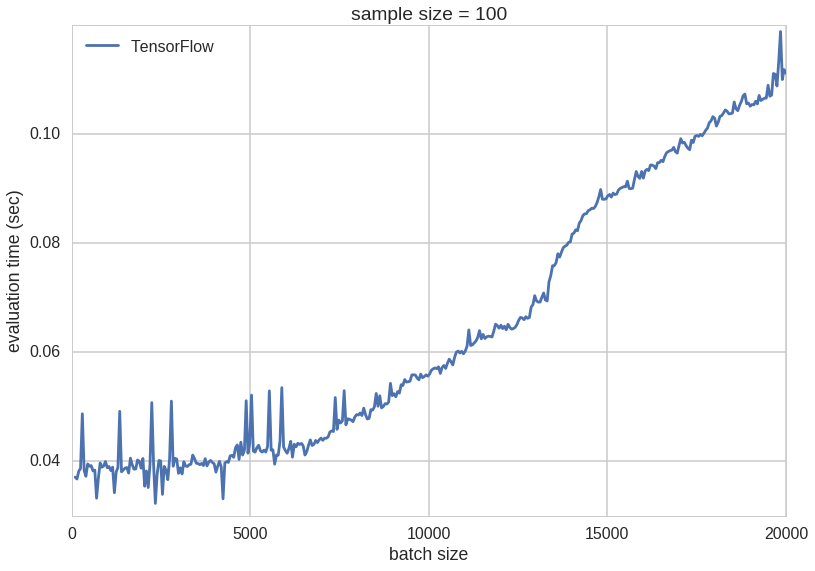
\includegraphics[width=.9\textwidth]{batch-tf-only}
%   \caption{Here only the TensorFlow implementation's evaluation time is depicted without the baseline. It reveals that under 2000 samples the process is nearly constant in time complexity. Above 2000 samples it starts to behave linearly, but it is important to mention that the slope of the fitting linear curve is significantly less steeper than the SciPy baseline.}
%   \label{fig:batch-tf-only}
% \end{figure}

\section{Time per sample}
Finally, we normalized the computation time with regards to the batch size, as a result we have a curve that tells that with fixed sample length at given batch size how much time does it take to evaluate a single entry. For a detailed benchmark see Figure \ref{fig:norm}.

\begin{figure}
  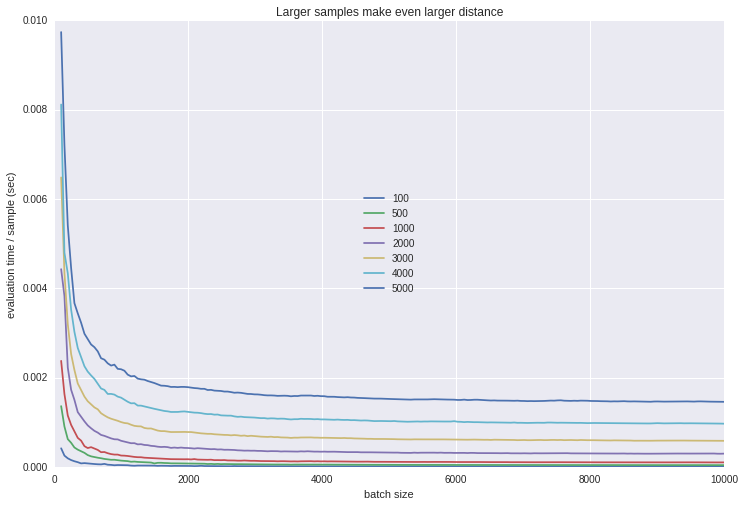
\includegraphics[width=.9\textwidth]{norm}
  \caption{This curve tells that with fixed sample length (different curves on the figure) at given batch size how much time does it take to evaluate a single entry.}
  \label{fig:norm}
\end{figure}

\clearpage

%% TARTALOM
%%%%%%%%%%%%%%%%%%%%%%%%%%%%%%%
%% BEFEJEZÉS

\clearpage
\input{content/summary}
\chapter{Future}

\paragraph{Short-term plans.} 
Currently I have a working version of the convolutional layer, 
however the implementation still relies on \texttt{convolve2d} function of ScyPy, which slows down the training process.
In the following months I will work on my own implementation of the convolution function, 
and improve the network usability.
Recently I have been able to train my network on CIFAR~\cite{cifar}, and ImageNET~\cite{deng2009imagenet} dataset, and the results are encouraging, however not enough yet to publish.
I am also working on \emph{Restrictive Boltzmann Machines} to be able to build and make experiments of \emph{Deep Belief} networks.

I am very interested in fields of \emph{Reinforcement Learning}, 
and I plan to utilize a network that plays the popular game, \texttt{agar-io}.
Also I am currently studying \emph{Recurrent Neural Networks} especially implementations of \emph{Long Short-Term Memory} architectures, 
which are not just better for audio recognition tasks, but can be used as Generative networks, producing artificial samples.
I want to create an application capable of accompanying musicians in jam-sessions, based on \emph{LSTM} networks.
I will continue my studies in field of \emph{Generative Adversarial Networks} which is currently a very hot topic of Computer Vision.

\paragraph{Long-term plans}
My studies have two basic motivation:
When observing living organisms I think about how could we model them, 
and reverse-engineer their function. 
On the other hand, I want to get closer to understand our 
environment and how can we build knowledge based on our experiences.
I believe, that one day my studies in Neuroscience and Artifical Intelligence will converge to a common point, and I will be able to model cognitive functions of the human mind.

\clearpage

\addcontentsline{toc}{chapter}{List of Figures}
\clearpage

\printbibliography
\addcontentsline{toc}{chapter}{Bibliography}
\clearpage
%% BEFEJEZÉS
%%%%%%%%%%%%%%%%%%%%%%%%%%%%%%%
\end{document}
